%% LyX 1.5.5 created this file.  For more info, see http://www.lyx.org/.
%% Do not edit unless you really know what you are doing.
\documentclass[twocolumn,french]{IEEEtran}
\usepackage[T1]{fontenc}

\usepackage{graphicx}
\usepackage{babel}
\usepackage{color}

\newtheorem{quest}{Question}

\addtolength{\hoffset}{2cm}
\addtolength{\textwidth}{-2cm}
\addtolength{\textheight}{-2cm}
\addtolength{\voffset}{2cm}


\newif\ifComment \Commenttrue        % POUR BASCULER EN MODE sans commentaire
%\newif\ifComment \Commentfalse    % POUR BASCULER EN MODE  comment�


\ifComment
  \newcommand{\Comment}[1]{} % blachit les lettres pour les rendres invisibles
\else
  \newcommand{\Comment}[1]{\vspace{1cm}\color{blue} \textsl{Commentaire :  {#1} } \color{black} }
\fi








\begin{document}

\title{TD1  Asm Cortex-M3\\Premier sujet de TD}

\author{3 IMACS 2010-2011 \\ \vspace{.5 cm} \small{Vincent MAHOUT}}

\maketitle
\begin{abstract}
Le but de ce TD est tout d'abord de comprendre un petit bout de code. Cela suppose donc de voir comment l'encha�nement d'instructions basiques permettent de construire un algorithme simple. Une aspect important de compr�hension concerne l'acc�s en m�moire par indirection. Enfin, il s'agira de jouer sur ces modes d'adressage afin de modifier le code dans l'espoir de l'optimiser.
\end{abstract}


\section{Le programme}

Soit le morceau de programme suivant :

\begin{figure}[h]
    \begin{center}
      % Requires \usepackage{graphicx}
      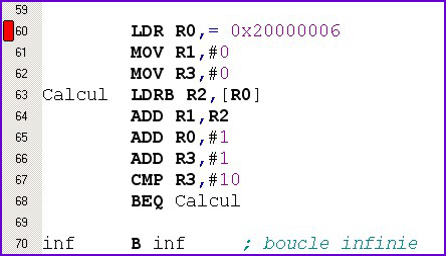
\includegraphics[width=0.5\textwidth]{Listing.jpg}
      \caption{Premier listing}
    \end{center}
\end{figure}

Lors de l'ex�cution de ce code la m�moire aura le contenu suivant :

\begin{figure}[h]
    \begin{center}
      % Requires \usepackage{graphicx}
      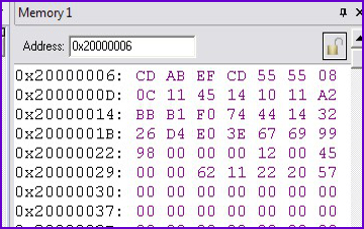
\includegraphics[width=0.5\textwidth]{memoire.jpg}
      \caption{Contenu m�moire}
    \end{center}
\end{figure}


\section{comprehension}
Dans un premier temps, il s'agit d'analyser ce programme.


\Comment{leur faire reprendre la notion du test conditionn�....vu rapidement en cours....insister sur le fait qu'un cmp tout seul ne sert � rien}

\begin{quest}
Que font les deux lignes \emph{CMP R3,\#10} et \emph{BEQ Calcul}? - Que peut -on en d�duire sur le d�roulement du programme ?
\end{quest}


\Comment{la structuration algo n'est pas encore vue en cours - faire extraire un organigramme pour introduire cela....}
\begin{quest}
D�terminez ce que fait ce petit programme en extrayant son organigramme g�n�ral.
\end{quest}

\section{Adressage m�moire}

\Comment{adressage indirect assez d�taill� en cours. Cela ne doit poser pb qu'aux absents !!! }
\begin{quest}
Remplissez le tableau relatant l'�tat des registres \emph{R0} � \emph{R3} (en hexad�cimal) � chaque fois que \emph{PC} passe sur l'�tiquette \emph{Calcul}.
\end{quest}

\begin{center}
\begin{tabular}{|c|c|c|c|c|}
  \hline
  % after \\: \hline or \cline{col1-col2} \cline{col3-col4} ...
    & R0  & R1  & R2  & R3  \\
\hline
\hline
1    &\hspace{1cm}   & \hspace{1cm}  & \hspace{1cm}  & \hspace{1cm}  \\
\hline
2    &   &   &   &   \\
\hline
3    &   &   &   &   \\
\hline
4    &   &   &   &   \\
\hline
5    &   &   &   &   \\
\hline
6    &   &   &   &   \\
\hline
7    &   &   &   &   \\
\hline
8    &   &   &   &   \\
\hline
9    &   &   &   &   \\
\hline
10    &   &   &   &   \\
  \hline
\end{tabular}
\end{center}


\Comment{reprendre la notion qu'en assembleur il n'y a pas de type de donn�es jsute des quantit�s d'octets � charger => modiifcaiton de l'incr�mentation du pointeur ...Attention un int est a priori sign� donc l'instruction de chargement est LDRSH ... }

\begin{quest}
Le programmeur s'est tromp� dans son codage. En effet, le tableau contient 5 \textit{short int} (2 octets) et non 10 \textit{char} (1 seul octet). Modifiez les instructions pour apporter cette correction.
\end{quest}

\Comment{reprendre l'inversion pf PF de sdonnes en m�moire pour faire l'addition correctement}
\begin{quest}
Cette modification prise en compte, que vaudra le registre \emph{R1} lorsque \emph{PC} pointera sur  l'�tiquette \emph{inf} ?
\end{quest}

\section{Optimisation du code}

\Comment{reprendre le post d�placement...et son int�r�t pour ne plus g�rer l'incr�mentation du pointeur - 1 ligne de code en mois}
\begin{quest}
Modifiez la gestion du pointeur \emph{R0} pour utiliser un adressage indirect avec post-d�placement.
\end{quest}

\Comment{il n'y a pas de codage unique - d�cr�menter plut�t qu'incr�menter est souvent plu sjudicieix car cela permet d'utiliser le drapeau Z }
\begin{quest}
Modifiez le code pour supprimer l'instruction \emph{CMP} en se rappelant que l'instruction \emph{SUBS} modifie l'�tat du fanion \emph{Z}.
\end{quest}



\end{document}
